\documentclass[aspectratio=169, 12pt]{beamer}

% ── Theme & colours ──────────────────────────────────────────
\usetheme{Madrid}
\usecolortheme{seahorse}
\setbeamertemplate{navigation symbols}{}
\setbeamertemplate{footline}{%
  \hfill\insertframenumber/\inserttotalframenumber\hspace*{4pt}\vspace{2pt}}

\usepackage[utf8]{inputenc}
\usepackage[T1]{fontenc}
\usepackage{booktabs}
\usepackage{graphicx}
\usepackage{amsmath}
\usepackage{tikz}
\usetikzlibrary{arrows.meta, positioning, calc}
\usepackage{xcolor}

\definecolor{improvement}{RGB}{34,139,34}
\definecolor{failure}{RGB}{180,40,40}
\definecolor{neutral}{RGB}{80,80,80}

% ── Meta ─────────────────────────────────────────────────────
\title{Citation Recommendation with\\Hybrid Retrieval and Rank Fusion}
\subtitle{CodaBench Scientific Article 2025--2026}
\author{Martin}
\date{\today}

\begin{document}

% ═══════════════════════════════════════════════════════════════
% SLIDE 1 — Title
% ═══════════════════════════════════════════════════════════════
\begin{frame}
\titlepage
\end{frame}

% ═══════════════════════════════════════════════════════════════
% SLIDE 2 — The Challenge
% ═══════════════════════════════════════════════════════════════
\begin{frame}{The Challenge: Citation Recommendation}
\textbf{Task.} Given a scientific paper (the \emph{query}), retrieve the papers
it should cite from a corpus of 20\,000 articles.

\vspace{0.6em}
\begin{itemize}
    \item Each query paper has a title, abstract, body text, and metadata
    \item Ground truth: actual citation lists from published papers
    \item Multi-domain: Biology, Medicine, Computer Science, Physics, Chemistry\ldots
    \item Not topical similarity --- \emph{citation proximity}:
          ``would paper A cite paper B?''
\end{itemize}

\vspace{0.6em}
\textbf{Constraint:} 8\,GB VRAM (WSL), so large cross-encoders and
billion-parameter models are out of scope.
\end{frame}

% ═══════════════════════════════════════════════════════════════
% SLIDE 3 — Dataset & Evaluation
% ═══════════════════════════════════════════════════════════════
\begin{frame}{Dataset \& Evaluation}
\begin{columns}[T]
\begin{column}{0.48\textwidth}
\textbf{Data}
\begin{itemize}
    \item \textbf{Corpus}: 20\,000 papers (Parquet)
    \item \textbf{Public queries}: 100 papers with ground-truth citations
    \item \textbf{Held-out queries}: unlabelled, for CodaBench submission
    \item Fields: \texttt{title}, \texttt{abstract}, \texttt{full\_text},
          \texttt{chunk\_meta}, \texttt{domain}
\end{itemize}
\end{column}
\begin{column}{0.48\textwidth}
\textbf{Metrics}
\begin{itemize}
    \item \textbf{NDCG@10} (primary --- leaderboard ranking)
    \item Recall@$k$ ($k=10, 100$)
    \item Precision@$k$
    \item MRR@10
    \item MAP
\end{itemize}
\vspace{0.4em}
\footnotesize Noise floor $\approx \pm 0.005$ NDCG@10 with 100 queries.
\end{column}
\end{columns}
\end{frame}

% ═══════════════════════════════════════════════════════════════
% SLIDE 4 — Final Architecture Overview
% ═══════════════════════════════════════════════════════════════
\begin{frame}{System Architecture (Final)}
\centering
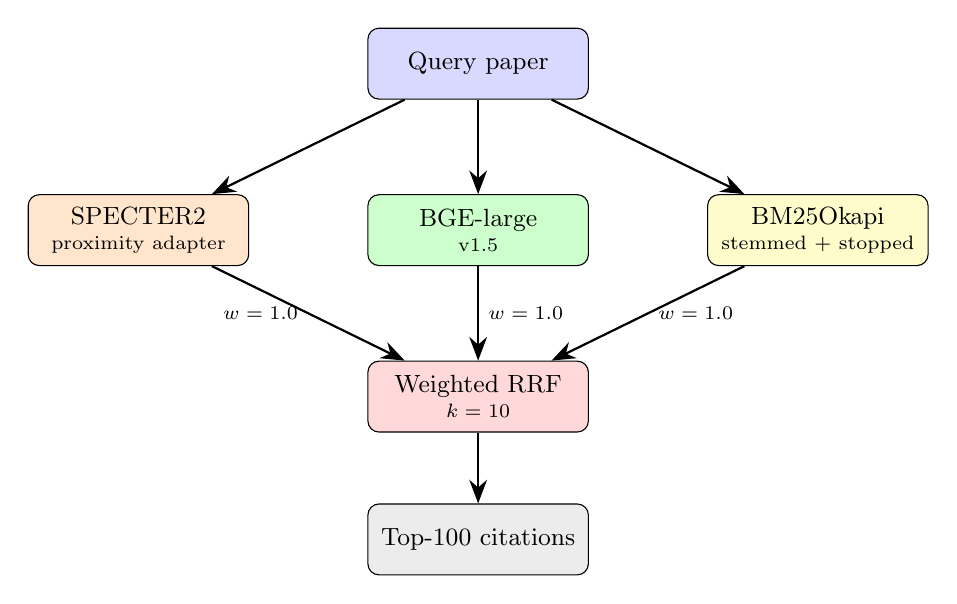
\begin{tikzpicture}[
    node distance=1.2cm and 2.2cm,
    block/.style={draw, rounded corners, minimum width=2.8cm,
                  minimum height=0.9cm, align=center, font=\small},
    arrow/.style={-{Stealth[length=3mm]}, thick},
]
    % Query
    \node[block, fill=blue!15] (query) {Query paper};

    % Three retrievers
    \node[block, fill=orange!20, below left=1.2cm and 1.5cm of query]  (specter) {SPECTER2\\[-2pt]\scriptsize proximity adapter};
    \node[block, fill=green!20,  below=1.2cm of query]                 (bge)     {BGE-large\\[-2pt]\scriptsize v1.5};
    \node[block, fill=yellow!20, below right=1.2cm and 1.5cm of query] (bm25)    {BM25Okapi\\[-2pt]\scriptsize stemmed + stopped};

    % RRF
    \node[block, fill=red!15, below=1.2cm of bge] (rrf) {Weighted RRF\\[-2pt]\scriptsize $k=10$};

    % Top-100
    \node[block, fill=gray!15, below=0.9cm of rrf] (out) {Top-100 citations};

    % Arrows
    \draw[arrow] (query) -- (specter);
    \draw[arrow] (query) -- (bge);
    \draw[arrow] (query) -- (bm25);
    \draw[arrow] (specter) -- node[left, font=\scriptsize] {$w=1.0$} (rrf);
    \draw[arrow] (bge)     -- node[right, font=\scriptsize] {$w=1.0$} (rrf);
    \draw[arrow] (bm25)    -- node[right, font=\scriptsize] {$w=1.0$} (rrf);
    \draw[arrow] (rrf) -- (out);
\end{tikzpicture}
\end{frame}

% ═══════════════════════════════════════════════════════════════
% SLIDE 5 — Baseline
% ═══════════════════════════════════════════════════════════════
\begin{frame}{Step 0: Dense Baseline}
\textbf{Setup.} Single dense encoder (BGE-large-en-v1.5).\\
Input: \texttt{title + abstract}, cosine similarity, no fusion.

\vspace{0.8em}
\begin{center}
\Large NDCG@10 $\approx$ \textbf{0.50}
\end{center}

\vspace{0.8em}
\textbf{Diagnosis:}
\begin{itemize}
    \item MRR@10 $\approx 0.72$ --- rank-1 paper was usually correct
    \item But the 2\textsuperscript{nd}--5\textsuperscript{th} relevant papers
          were scattered between ranks 6 and 30
    \item Problem was \emph{ordering}, not candidate generation
\end{itemize}
\end{frame}

% ═══════════════════════════════════════════════════════════════
% SLIDE 6 — SPECTER2
% ═══════════════════════════════════════════════════════════════
\begin{frame}{Improvement 1: SPECTER2 with Proximity Adapter}
\textbf{Idea.} Replace generic encoder with a \emph{citation-trained} model.

\vspace{0.4em}
\begin{itemize}
    \item \texttt{allenai/specter2\_base} + \texttt{proximity} adapter
    \item Trained on citation triplets from Semantic Scholar
    \item Input format: \texttt{"title [SEP] abstract"}, CLS pooling, L2-normalised
\end{itemize}

\vspace{0.6em}
\begin{center}
\large NDCG@10: 0.50 $\rightarrow$ \textcolor{improvement}{\textbf{0.54}} \quad
\textcolor{improvement}{(+0.04)}
\end{center}

\vspace{0.4em}
\textbf{Why it works:} SPECTER2's training objective is ``papers that cite each
other should be close'' --- exactly our task.
\end{frame}

% ═══════════════════════════════════════════════════════════════
% SLIDE 7 — BM25 + RRF
% ═══════════════════════════════════════════════════════════════
\begin{frame}{Improvement 2: Hybrid with BM25 (Weighted RRF)}
\textbf{Problem.} Dense encoders miss exact lexical matches:
author surnames, dataset names, method acronyms.

\vspace{0.4em}
\textbf{Solution.} Add BM25Okapi (Porter-stemmed, stopword-filtered) and fuse
via \textbf{Reciprocal Rank Fusion}:

\vspace{0.3em}
\[
\text{score}(d) = \sum_{r \in \text{retrievers}} \frac{w_r}{k + \text{rank}_r(d)}
\qquad k = 10
\]

\vspace{0.3em}
Grid search: $w_{\text{bm25}} \in \{0.3, 0.5, 0.7, 1.0\}$, best = \textbf{0.5}

\vspace{0.6em}
\begin{center}
\large NDCG@10: 0.54 $\rightarrow$ \textcolor{improvement}{\textbf{0.568}} \quad
\textcolor{improvement}{(+0.028)}
\end{center}
\end{frame}

% ═══════════════════════════════════════════════════════════════
% SLIDE 8 — Body chunks
% ═══════════════════════════════════════════════════════════════
\begin{frame}{Improvement 3: Body-Chunk Enrichment}
\textbf{Problem.} \texttt{title + abstract} discards the entire paper body.

\vspace{0.4em}
\textbf{Solution.} Append the first body chunks ($\geq$50 chars each) to the
document representation for both SPECTER2 and BM25.

\vspace{0.4em}
\begin{itemize}
    \item SPECTER2 still truncates at 512 tokens --- but the \emph{first} chunk
          often contains key method/dataset names
    \item BM25 indexes \emph{all} appended text --- captures terms that never
          appear in abstracts
\end{itemize}

\vspace{0.6em}
\begin{center}
\large NDCG@10: 0.568 $\rightarrow$ \textcolor{improvement}{\textbf{0.577}} \quad
\textcolor{improvement}{(+0.009)}
\end{center}
\end{frame}

% ═══════════════════════════════════════════════════════════════
% SLIDE 9 — BGE as second dense
% ═══════════════════════════════════════════════════════════════
\begin{frame}{Improvement 4: BGE-large as a Second Dense Retriever}
\textbf{Idea.} Two dense models that \emph{disagree} are better than two that agree.

\vspace{0.4em}
\begin{itemize}
    \item \textbf{SPECTER2}: citation proximity (``cited together'')
    \item \textbf{BGE-large}: general semantic similarity (``about the same topic'')
    \item Complementary signals $\Rightarrow$ 3-way weighted RRF
\end{itemize}

\vspace{0.4em}
Weights: SPECTER2 = 1.0, BGE = 1.0, BM25 = 0.5

\vspace{0.6em}
\begin{center}
\large NDCG@10: 0.577 $\rightarrow$ \textcolor{improvement}{\textbf{0.585}}
\quad \textcolor{improvement}{(+0.008)}\\[4pt]
\normalsize CodaBench: \textbf{0.60}
\end{center}
\end{frame}

% ═══════════════════════════════════════════════════════════════
% SLIDE 10 — Wider pool
% ═══════════════════════════════════════════════════════════════
\begin{frame}{Improvement 5: Wider Pool + More Body Chunks}
Two targeted hyperparameter changes:

\vspace{0.4em}
\begin{itemize}
    \item \textbf{Retrieval pool}: 200 $\rightarrow$ 300 candidates per retriever
    \item \textbf{Body chunks}: 3 $\rightarrow$ 6 chunks per document
\end{itemize}

\vspace{0.4em}
Grid search shifted optimal BM25 weight from 0.5 to \textbf{1.0} ---
with more body text, BM25 becomes as informative as the dense retrievers.

\vspace{0.6em}
\begin{center}
\large NDCG@10: 0.585 $\rightarrow$ \textcolor{improvement}{\textbf{0.587}}
\quad \textcolor{improvement}{(+0.002)}\\[4pt]
\normalsize Final weights: SPECTER2 = 1.0, BGE = 1.0, BM25 = 1.0
\end{center}
\end{frame}

% ═══════════════════════════════════════════════════════════════
% SLIDE 11 — What didn't work
% ═══════════════════════════════════════════════════════════════
\begin{frame}{What Did NOT Work (and Why)}
\begin{columns}[T]
\begin{column}{0.48\textwidth}
\textbf{\textcolor{failure}{Jina-embeddings-v3}}\\[4pt]
\small
2048-token context, top of MTEB.\\
Result: NDCG@10 = 0.573 \textcolor{failure}{($-$0.012)}

\vspace{0.4em}
\textbf{Why:} Optimised for web/multilingual retrieval.
Citation proximity $\neq$ topical similarity.
Longer context doesn't help with the wrong objective.
\end{column}
\begin{column}{0.48\textwidth}
\textbf{\textcolor{failure}{SciNCL as 4\textsuperscript{th} retriever}}\\[4pt]
\small
Citation-trained like SPECTER2.\\
Result: $\Delta = -0.004$ \textcolor{failure}{(within noise)}

\vspace{0.4em}
\textbf{Why:} Trained on the \emph{same signal} as SPECTER2.
Fusion gains come from \textbf{disagreement} ---
stacking near-duplicates adds nothing.
\end{column}
\end{columns}

\vspace{0.8em}
\begin{center}
\fbox{\parbox{0.8\textwidth}{\centering
\textbf{Lesson:} MS MARCO-trained and redundant-signal components consistently
fail on citation recommendation. Only citation-aware + general semantic + lexical
provides effective diversity.}}
\end{center}
\end{frame}

% ═══════════════════════════════════════════════════════════════
% SLIDE 12 — Progression chart
% ═══════════════════════════════════════════════════════════════
\begin{frame}{NDCG@10 Progression}
\centering
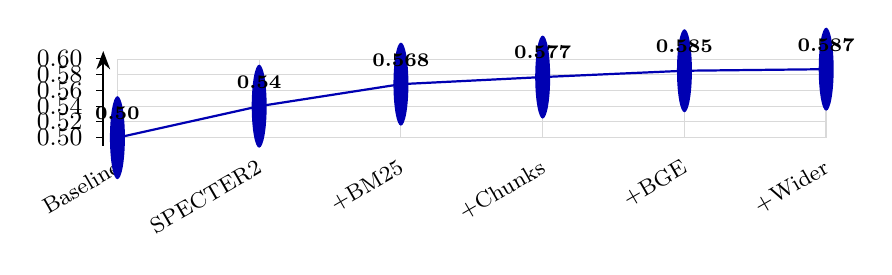
\begin{tikzpicture}[xscale=1.8, yscale=10]
    % Grid
    \draw[gray!30, thin] (0, 0.50) grid[xstep=1, ystep=0.02] (5, 0.60);

    % Y axis
    \draw[thick, -{Stealth}] (-0.1, 0.49) -- (-0.1, 0.61);
    \foreach \y in {0.50, 0.52, 0.54, 0.56, 0.58, 0.60} {
        \draw (-0.15, \y) -- (-0.1, \y) node[left=4pt, font=\small] {\y};
    }

    % X axis labels
    \foreach \x/\lab in {
        0/{Baseline},
        1/{SPECTER2},
        2/{+BM25},
        3/{+Chunks},
        4/{+BGE},
        5/{+Wider}} {
        \node[below, font=\footnotesize, rotate=30, anchor=north east] at (\x, 0.49) {\lab};
    }

    % Data points and lines
    \coordinate (p0) at (0, 0.500);
    \coordinate (p1) at (1, 0.540);
    \coordinate (p2) at (2, 0.568);
    \coordinate (p3) at (3, 0.577);
    \coordinate (p4) at (4, 0.585);
    \coordinate (p5) at (5, 0.587);

    \draw[thick, blue!70!black]
        (p0) -- (p1) -- (p2) -- (p3) -- (p4) -- (p5);

    \foreach \p in {p0, p1, p2, p3, p4, p5}
        \fill[blue!70!black] (\p) circle (1.5pt);

    % Annotations
    \node[above=3pt, font=\scriptsize\bfseries] at (p0) {0.50};
    \node[above=3pt, font=\scriptsize\bfseries] at (p1) {0.54};
    \node[above=3pt, font=\scriptsize\bfseries] at (p2) {0.568};
    \node[above=3pt, font=\scriptsize\bfseries] at (p3) {0.577};
    \node[above=3pt, font=\scriptsize\bfseries] at (p4) {0.585};
    \node[above=3pt, font=\scriptsize\bfseries] at (p5) {0.587};
\end{tikzpicture}
\end{frame}

% ═══════════════════════════════════════════════════════════════
% SLIDE 13 — Key Takeaways
% ═══════════════════════════════════════════════════════════════
\begin{frame}{Key Takeaways}
\begin{enumerate}
    \item \textbf{Task-aligned models matter most.}
          SPECTER2 (citation-trained) gave the single biggest jump (+0.04).
          Generic MTEB winners (Jina) underperformed.

    \vspace{0.4em}
    \item \textbf{Fusion gains come from disagreement.}
          SPECTER2 + BGE + BM25 each capture a different signal.
          Adding a 4\textsuperscript{th} model that agrees with an existing one
          (SciNCL $\approx$ SPECTER2) adds nothing.

    \vspace{0.4em}
    \item \textbf{More text surface helps --- up to a point.}
          Body chunks improved BM25 substantially.
          Beyond 6 chunks, returns diminished.

    \vspace{0.4em}
    \item \textbf{Weighted RRF is simple and effective.}
          One hyperparameter per retriever, robust to tuning,
          no learned weights to overfit on 100 queries.
\end{enumerate}
\end{frame}

% ═══════════════════════════════════════════════════════════════
% SLIDE 14 — Thank you
% ═══════════════════════════════════════════════════════════════
\begin{frame}
\centering
\vspace{2cm}
{\Large Thank you}

\vspace{1.5cm}
\begin{tabular}{rl}
\textbf{Best local NDCG@10} & 0.587 \\
\textbf{Best CodaBench NDCG@10} & 0.60 \\
\textbf{Models} & SPECTER2, BGE-large, BM25Okapi \\
\textbf{Fusion} & Weighted Reciprocal Rank Fusion \\
\end{tabular}
\end{frame}

\end{document}
